\documentclass[aspectratio=169,11pt]{beamer}

\usetheme{Madrid}
\usecolortheme{default}
\setbeamertemplate{navigation symbols}{}
\setbeamertemplate{footline}[frame number]

\usepackage{amsmath}
\usepackage{booktabs}
\usepackage{graphicx}

\title{Semiparametric SDF Estimators\\for Pooled, Non-Traded Cash Flows}
\subtitle{GOR AG Analytics Workshop, Frankurt (Deutsche Bahn)}
\author{Christian Tausch, Alexander Bohnert}
\institute{AssetMetrix GmbH, Hochschule M{\"u}nchen}
\date{March 6, 2026}

\begin{document}

\begin{frame}
  \titlepage
\end{frame}

\begin{frame}{Guiding Question}
	\begin{center}
		\includegraphics[width=0.95\linewidth]{images/TR1.png}
	\end{center}
	\footnotesize Source: \url{https://traderepublic.com/en-de/private-markets}
\end{frame}

\begin{frame}{Guiding Question}
	\begin{center}
		\includegraphics[width=0.88\linewidth]{images/TR2.png}
	\end{center}
	\footnotesize Source: \url{https://traderepublic.com/en-de/private-markets}
\end{frame}

\begin{frame}{Guiding Question}
	\begin{center}
		\includegraphics[width=0.88\linewidth]{images/TR3.png}
	\end{center}
	\footnotesize Source: \url{https://traderepublic.com/en-de/private-markets}
\end{frame}

\begin{frame}{Guiding Question}
	
	\emph{Are private markets really not connected to public market volatility?}
	\vspace{1.6em}
	
	\textbf{How can we estimate the true public-market exposure of private equity funds?}
	
	\vspace{0.6em}
	\begin{itemize}
		\item Target: recover latent market exposure from non-traded PE cash flow/NAV data.
		\item Challenge: stale NAVs, asynchronous cash flows, and overlapping fund lives.
		\item Plan: naive approach first, then semiparametric SDF estimation.
	\end{itemize}
	
	\vspace{0.6em}
	\textbf{Useful for:}
	
	\begin{itemize}
		\item Risk-adjusted benchmarks for private equity funds.
		\item Holistic risk management for public and private portfolios.
		\item More realistic strategic asset allocation decisions.
	\end{itemize}
\end{frame}



\begin{frame}{Agenda}
\begin{enumerate}
  \item Motivation: NAV-return autocorrelation
  \item Estimation framework
  \item Simulation evidence
  \item Empirical PE results
  \item Takeaways
\end{enumerate}
\end{frame}

\begin{frame}[t]{Motivation: Public Returns vs Private Cash Flows}
\begin{center}
\includegraphics[width=0.90\linewidth]{figures/motivating_public_vs_private.pdf}
\end{center}

\end{frame}

\begin{frame}{Motivation: \cite{D79} Regression from NAV Returns}
\begin{center}
\includegraphics[width=0.93\linewidth]{figures/motivating_nav_acf_dimson.pdf}
\end{center}
\vspace{-0.4em}
\scriptsize Data: Preqin quarterly index levels and q5 monthly $R_{MKT}$ aggregated to quarters (overlap through 2022Q4).
\end{frame}

\begin{frame}{Estimator: Starting Point \cite{DLP12}}
\small
For each fund $i$, \cite{DLP12} imposes a zero-NPV pricing condition at inception date $\tau_i^{(0)}$:
\[
\epsilon_i^{\text{DLP}}(\theta)=\sum_t \Psi_{\tau_i^{(0)},t}(\theta)\,CF_{i,t}
\]

Cross-sectional estimator:
\[
\hat\theta_{\text{DLP}}=\arg\min_{\theta\in\Theta}\frac{1}{n}\sum_{i=1}^n\left(\epsilon_i^{\text{DLP}}(\theta)\right)^2
\]

\vspace{0.2em}
\textbf{Mapping to our notation}
\begin{itemize}
  \item DLP12 is the special case $\mathcal{T}_i=\{\tau_i^{(0)}\}$, so $|\mathcal{T}_i|=1$.
  \item Then $\bar\epsilon_i(\theta)=\epsilon_i^{\text{DLP}}(\theta)$ and the LMD objective nests DLP12.
  \item This paper extends DLP12 by allowing multiple discount dates per fund ($|\mathcal{T}_i|>1$).
\end{itemize}
\vspace{0.15em}
{\tiny Variables: $i$ fund/portfolio index, $t$ cash-flow time, $\tau_i^{(0)}$ inception discount date, $CF_{i,t}$ net cash flow, $\Psi_{\tau,t}(\theta)$ SDF ratio, $\theta$ parameter vector, $\Theta$ parameter space, $n$ number of units.}
\end{frame}

\begin{frame}{Estimator: Least Mean Distance (LMD)}
For fund $i$ and discounting date $\tau$:
\[
\epsilon_{\tau,i}(\theta)=\sum_t \Psi_{\tau,t}(\theta)\,CF_{i,t}
\]

Average over selected discounting dates $\mathcal{T}_i$:
\[
\bar\epsilon_i(\theta)=\frac{1}{|\mathcal{T}_i|}\sum_{\tau\in\mathcal{T}_i}\epsilon_{\tau,i}(\theta)
\]

Estimate parameters by nonlinear least-mean-distance:
\[
\hat\theta=\arg\max_{\theta\in\Theta}\left(-\frac{1}{n}\sum_{i=1}^n L(\bar\epsilon_i(\theta))\right),\quad L(x)=x^2
\]
\vspace{0.25em}
{\tiny Variables: $i$ fund/portfolio index, $t$ cash-flow time, $\tau$ discounting date, $CF_{i,t}$ net cash flow, $\Psi_{\tau,t}(\theta)$ SDF ratio, $\theta$ parameter vector, $\mathcal{T}_i$ discount-date set.}
\end{frame}

\begin{frame}[t]{Estimator: Net Present Value (NPV) vs Net Future Value (NFV)}
\begin{itemize}
  \item NPV-only discounting (fund inception) is theoretically unbiased.
  \item NFV: Adding future-value dates introduces a timing risk \textbf{bias} term.
  \item \textbf{But:} Finite-sample performance can improve when averaging across dates.
\end{itemize}

\begin{center}
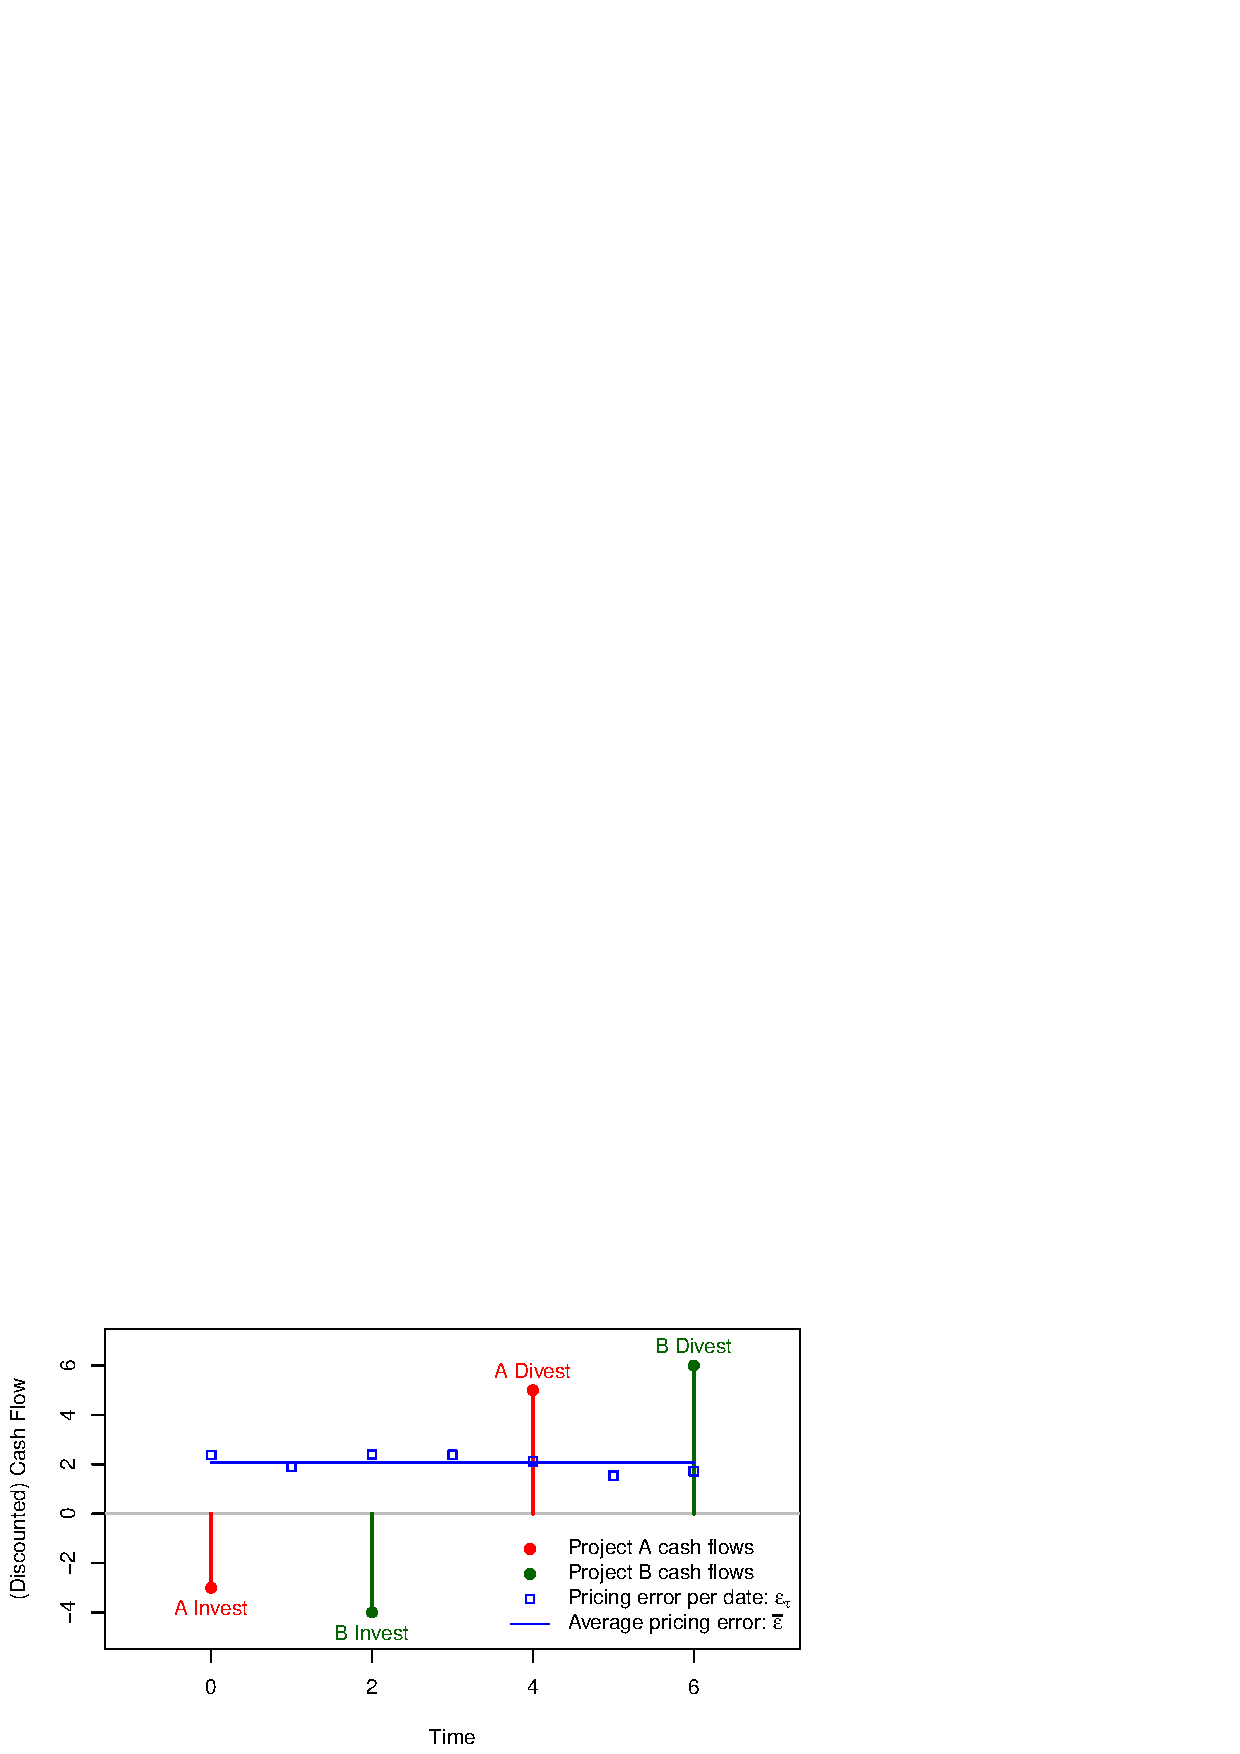
\includegraphics[width=0.63\linewidth]{figures/npvs3.pdf}
\end{center}
\end{frame}

\begin{frame}{Simulation: What Is Tested?}
\begin{itemize}
  \item \textbf{Base:} 20 vintages, synthetic fund cash flows generated under known SDF structure.
  \item \textbf{Focus on horizon choice:} size of discounting set $\mathcal{T}$.
  \item \textbf{Compare units:} individual funds vs vintage-year portfolios (VYP).
  \item \textbf{Compare sample geometry:} more vintages ($V$) vs larger within-vintage size ($n/V$).
  \item \textbf{Compare model forms:} simple linear vs exponential affine SDF.
\end{itemize}
\end{frame}

\begin{frame}[t]{Simulation: 1.\ Single Funds vs Portfolio Formation}
\begin{center}
\includegraphics[width=0.8\linewidth]{figures/bias_comparison1.pdf}
\end{center}

\textbf{Takeaway:} vintage-year portfolios materially reduce bias and variance versus single-fund estimation.
\end{frame}

\begin{frame}{Simulation: 2.\ More Vintages or More Funds per Vintage?}
\begin{center}
\includegraphics[width=0.82\linewidth]{figures/bias_comparison3.pdf}
%\includegraphics[width=0.49\linewidth]{figures/bias_comparison2.pdf}
\end{center}

\textbf{Takeaway:} increasing funds per vintage is more powerful for variance reduction than only extending the time span.
\end{frame}

\begin{frame}[t]{Simulation: 3.\ Linear vs Exponential Affine SDF}
\begin{center}
\includegraphics[width=0.82\linewidth]{figures/bias_comparison5.pdf}
\end{center}

\textbf{Takeaway:} no robust finite-sample superiority of exponential affine specification in this setting.

\cite{KN16}
\end{frame}

\begin{frame}{Simulation: Synthesis}
\begin{enumerate}
  \item Use portfolio aggregation to stabilize estimation.
  \item Prioritize richer cross-sections per vintage when possible (more funds per moment).
  \item Prefer parsimonious factor structure in current PE data regime.
  \item Horizon choice (size of $\mathcal{T}$) is a first-order control for finite-sample performance.
\end{enumerate}

\vspace{0.4em}
\textbf{Interpretation:} practical estimator quality is dominated by finite-sample bias-variance tradeoffs.
\end{frame}

\begin{frame}{Empirical: Preqin PE Data \& $q^5$ Public Factors}
\begin{itemize}
  \item Data snapshot: 2745 PE funds, vintages 1983--2019.
  \item Primary unit for estimation: vintage-year portfolios (equal- and value-weighted).
  \item Factors: $q^5$ family; focus on MKT and simple two-factor extensions.
  \item Horizon selected from simulation guidance: 15-year baseline.
  \item Benchmark for comparison: NAV-based naive/Dimson market-exposure estimates from the motivation section.
\end{itemize}

\textbf{Singe-factor models:} Dimson beta as lower bound.

\textbf{Two-factor models:} Apply machine-learning methods to form ``stronger learner."
\end{frame}

\begin{frame}{Empirical: 1.\ Single-Factor MKT Model}
\begin{center}
\includegraphics[width=0.86\linewidth]{figures/empirical_PE_MKT.pdf}
\end{center}

\textbf{Reading:}
\begin{itemize}
  \item Short-horizon MKT betas are high and decline with horizon.
  \item Betas stabilize near 1 at long horizons.
  \item CV inference is much more stable than asymptotic $t$-statistics.
  \item Relative to naive contemporaneous NAV betas, SDF estimates are materially closer to full market exposure.
\end{itemize}
\end{frame}

\begin{frame}[t]{Empirical: 2.\ Two-Factor Models}
\begin{center}
\includegraphics[width=0.84\linewidth]{figures/empirical_PE_all_factors.pdf}
\end{center}

\textbf{Reading:}
\begin{itemize}
  \item Second-factor loadings vary strongly with horizon and weighting scheme.
  \item Most non-MKT factors do not show robust incremental signal.
\end{itemize}
\end{frame}

\begin{frame}{Empirical: 3.\ Vintage Cutoffs for Single-Factor Model}
\begin{center}
\includegraphics[width=1\linewidth]{figures/max_vintage_PE_MKT.pdf}
\end{center}

\textbf{Reading:} including newer vintages tends to increase estimated market exposure, with noisier asymptotic uncertainty.

\textbf{Dimson beta as lower bound!} 
\end{frame}

\begin{frame}{Empirical: 4.\ Vintage Cutoffs for Two-Factor Models}
	\begin{center}
		\includegraphics[width=1\linewidth]{figures/max_vintage_PE_all_factors.pdf}
	\end{center}
	
\end{frame}

\begin{frame}{Conclusion: What This Means for Practice and Research}
\textbf{For practitioners}
\begin{itemize}
  \item Start with parsimonious SDFs (MKT-first), then add complexity cautiously.
  \item Treat asymptotic significance alone as insufficient in sparse PE samples.
  \item Use dependence-aware validation (e.g., $hv$-block CV) as a default diagnostic.
\end{itemize}

\textbf{For researchers}
\begin{itemize}
  \item Finite-sample design choices can dominate asymptotic elegance.
  \item Data architecture (portfolio formation, horizon design) is part of identification.
\end{itemize}
\end{frame}

\begin{frame}{Conclusion: Main Takeaways}
\begin{enumerate}
  \item A semiparametric LMD framework can price pooled non-traded cash flows directly.
  \item The central empirical issue is finite-sample stability, not asymptotic theory alone.
  \item Portfolio aggregation and horizon design are key levers for usable inference.
  \item Current evidence supports single-factor MKT models as the robust baseline for PE.
  \item Naive contemporaneous NAV betas understate exposure; lag-aware methods partially recover it.
  \item Outlook: Multi-factor models can be stabilized by machine-learning techniques.
\end{enumerate}

\vspace{0.6em}
\centering
\Large Questions and Discussion
\end{frame}


\begin{frame}{Literature}


%% References
\bibliographystyle{apalike}
\bibliography{ref.bib}


\end{frame}


% Appendix





\begin{frame}{Backup: Comparison to DLP12 and KN16}
\small
\begin{tabular}{@{}p{0.18\linewidth}p{0.25\linewidth}p{0.25\linewidth}p{0.25\linewidth}@{}}
\toprule
& DLP12 & KN16 & This paper \\
\midrule
Estimator & Cross-sectional NLS & Time-series GMM (public SDF) & Nonlinear LMD \\
Cash flows priced & PE fund cash flows & Public replicating portfolios & PE fund cash flows \\
Discount dates & Inception only & Inception only & Flexible via $\mathcal{T}_i$ \\
Asymptotics & Infill & $V\to\infty$ & Increasing domain \\
Inference & Bootstrap & SHAC & SHAC + CV focus \\
\bottomrule
\end{tabular}
\end{frame}

\begin{frame}{Motivation: Why Measuring Risk Is Hard in Private Markets}
	\begin{itemize}
		\item PE funds generate \textbf{cash flow sequences}, not continuously traded returns.
		\item Fund lives overlap across vintages, creating dependence beyond standard panel assumptions.
		\item Fund valuation relies on reported NAVs, which can be stale/smoothed.
		\item Standard return-based factor models are not directly applicable.
	\end{itemize}
	
	\vspace{0.4em}
	\textbf{Implication:} we need a cash-flow-native SDF estimator with robust dependence-aware inference.
\end{frame}

\begin{frame}{Backup: Significant ACF Lags and Dimson Lag Choice}
\small
\begin{tabular}{lccc}
\toprule
Series & Significant lags in 1--8 & Consecutive from lag 1 & Dimson lag $L$ \\
\midrule
PE Global & 3 & 2 & 2 \\
PE North America & 5 & 3 & 3 \\
PE Europe & 3 & 2 & 2 \\
Buyout Global & 3 & 2 & 2 \\
Growth Global & 2 & 2 & 2 \\
VC Global & 5 & 5 & 5 \\
\bottomrule
\end{tabular}

\vspace{0.5em}
\textbf{Naive benchmark result:} contemporaneous beta is low ($\approx 0.32$--$0.39$), while Dimson beta increases to $\approx 0.63$--$0.96$.
\end{frame}

\begin{frame}[t]{Dependence Structure: Random Field View}
	\begin{itemize}
		\item Cross-sectional unit: fund or vintage-year portfolio.
		\item Dependence driven by economic proximity (here: vintage-year distance).
		\item Asymptotics: increasing domain ($V\to\infty$), bounded units per vintage.
	\end{itemize}
	
	\begin{center}
		\includegraphics[width=0.58\linewidth]{figures/randomfields.pdf}
	\end{center}
\end{frame}

\begin{frame}{Estimator: Inference Strategy}
	\begin{itemize}
		\item Asymptotic covariance: sandwich form $\Sigma=H^{-1}\Lambda H^{-1}$.
		\item Long-run dependence handled by SHAC (spatial HAC) with vintage-distance kernel.
		\item Small-sample reliability checked via \textbf{$hv$-block cross-validation}.
	\end{itemize}
	
	\vspace{0.4em}
	\textbf{Reason:} asymptotic approximations are fragile with only 20--40 vintage portfolios.
\end{frame}

\begin{frame}[t]{Simulation 4: Two-Factor q-Factor Models}
	\begin{center}
		\includegraphics[width=0.76\linewidth]{figures/bias_comparison4.pdf}
	\end{center}
	
	\textbf{Takeaway:} two-factor estimates are horizon-sensitive and high-variance; multivariate identification is fragile.
\end{frame}


\begin{frame}{Conclusion: Machine-Learning Ensembles}
	
	- Two-factor models are messy.
	
	- Idea: Combine multiple weak learners
	
	- Additionally estimate error term \cite{TP24}
	
\end{frame}







\end{document}
